        	\begin{question}{27}{Calcul}{1}{1223}
				Une droite passe par les points $A = (0;0)$ et $B = (2;3)$. Quelle est son équation?
            \end{question}
            \begin{reponses}
            	\item[true] $y(x)=\frac{3}{2}x$
            	\item[false] $y(x)=\frac{2}{3}x$
                \item[false] $y(x)=\frac{3}{2}x+1$
                \item[false] $y(x)=\frac{2}{3}x+1$
            \end{reponses}
			%%%%%%%%%%%%%%%%%%%%%%%%%%%%%%%%%%%%%
            \begin{question}{27}{Calcul}{2}{1223}
                Une droite passe par les points $A = (1;2)$ et $B = (5;7)$. Quelle est son équation?
            \end{question}
            \begin{reponses}
                \item[false] $y(x)=\num{0.8}x+\num{1.2}$
                \item[true] $y(x)=\num{1.25}x+\num{0.75}$
                \item[false] $y(x)=\num{0.75}x+\num{1.25}$
                \item[false] $y(x)=\num{1.2}x+\num{0.8}$
            \end{reponses}
            %%%%%%%%%%%%%%%%%%%%%%%%%%%%%%%%%%%%%
            \begin{question}{27}{Calcul}{2}{1223}
                Quelle est l'équation de la droite $AB$?\\
                \begin{center}
                	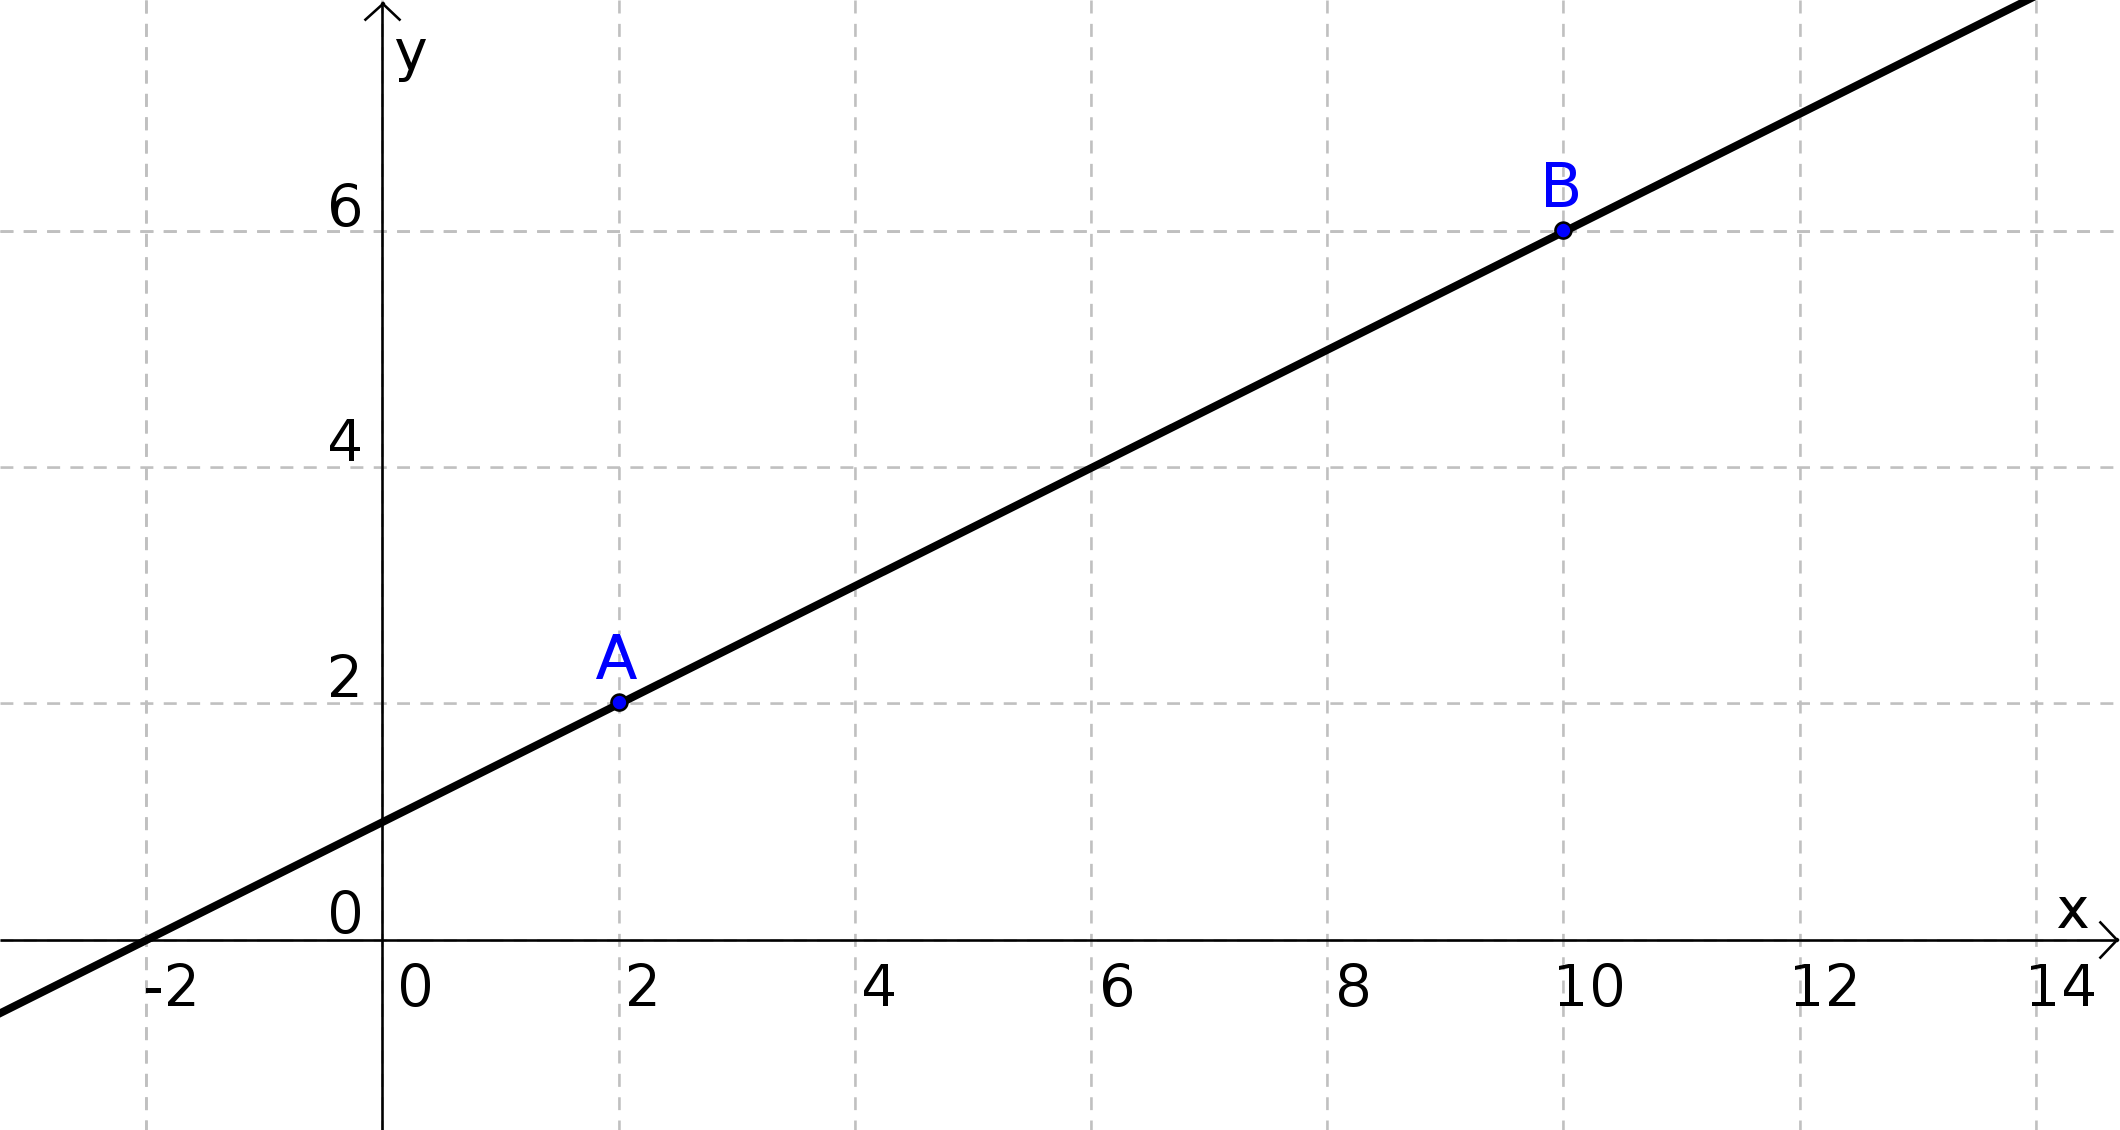
\includegraphics[width=0.5\textwidth]{Philippe/Figures_Philippe/calcul_6_9.png}
                \end{center}
            \end{question}
            \begin{reponses}
                \item[true] $y(x)=1/2x+1/2$
                \item[false] $y(x)=-2x+1/2$
                \item[false] $y(x)=1/2x-2$
                \item[false] $y(x)=x-1/2$
            \end{reponses}
            %%%%%%%%%%%%%%%%%%%%%%%%%%%%%%%%%%%%%
            \begin{question}{27}{Calcul}{2}{1223}
                En mesurant la vitesse d'un objet en chute libre à un temps $t=\SI{1}{\second}$ et $t=\SI{5}{\second}$, on trouve respectivement \SI{12}{\meter\per\second} et \SI{52}{\meter\per\second}. On sait que la vitesse d'un objet en chute libre dépend linéairement du temps (\textit{i.e.} $v(t) = a.t+b$). Que valent $a$ et $b$ dans ce cas?
            \end{question}
            \begin{reponses}
                \item[false] $a=2$ et $b=10$.
                \item[true] $a=10$ et $b=2$.
                \item[false] $a=8$ et $b=12$.
                \item[false] $a=12$ et $b=8$.
            \end{reponses}
            %%%%%%%%%%%%%%%%%%%%%%%%%%%%%%%%%%%%%
